
\chapter{MotoNeurons}
\label{chap:models-motoneurons}

Readers are recommended to read Chapter~\ref{chap:whole-cell-model} and
\ref{chap:neuron-models}. As pointed out by Rall, a mathematical model
is the need emerged from the three available information:
\begin{enumerate}
\item anatomical concept of neuron, together with the anatomical fact
  that extensive dendritic branching play a significant role in many
  neuron types
\item theoretical development of membrane model
\item quantitative electrophysiological data obtained from individual
  neuron by experimental technique (intracellular and extracellular
  electrodes)
\end{enumerate}
The earliest works to model neurons were targeted to
motoneurons. J.C. Eccles was one of the first to exploit this topic
(sect.~\ref{sec:stand-moton-eccl}). However, the more importance is
Wilfrid Rall's work with his 10-compartment model~\citep{rall1967dts}
which build the foundation for computational neurology, i.e. it can be
applied for any neuronal type (read Sect.~\ref{sec:ralls-model}). For
each particular type, it may require to change the values of the
parameters or to add explicit consideration of different sets of
dendrites (e.g. basal or apical in pyramidal cells).

Rall has taken into account the contribution of dendrite by building
the equivalent cable theory, allowing the qualitative interpretation
of subthreshold signal, i.e. based on postsynaptic potential we can
estimate how far out on the dendrite tree that synapse is located. 

Then, Dodge and Cooley extended Rall's work
(sect.~\ref{sec:dodge-cooley-model})

\section{Standard motoneuron of Eccles}
\label{sec:stand-moton-eccl}

This is one of the very first model of
motoneurons\citep{eccles1957pnc}. It models a cat motoneuron with a
spherical soma (70$\mu$m in diameter), and 6 dendrites of infinite
length with diameter $d=5\mu$m. 

A later revision added an axon ($d'=5\mu$m) to the
model~\citep{coombs1959ecm}. However, such models still underestimated
the dendritic contribution by a significant amount. Thus, the more
significant contribution is Rall's model when dendrite is modeled as
an equivalent cable.

\section{Rall's model (1967)}
\label{sec:ralls-model}

% As the voltage at the soma (body) can be measured experimentally with
% greater ease than those in dendrite network, and further, it is the
% voltage at the soma that determine whether or not the neuron fires an
% action potential. 

Chap.~\ref{chap:neuron-models} has described the general ideas of Rall
in building a representation for the branching dendrites, i.e.  cable
model (Sect.\ref{sec:cable_equation}). 

One of the major question is to know the solution, i.e.
the voltage, at the end of the cable that connects to the soma.  Rall first
proposed {\bf Rall lumped-soma model}~\citep{rall1967dts}.
\textcolor{red}{The idea of this model is not only applicable to
  motoneurons, but also to other types of nerve cells also}.

The assumptions, as shown in Fig.~\ref{fig:rall_lumpedmodel}:
\begin{enumerate}
\item The soma is isopotential (i.e. the membrane potential is the
  same as all points)

\item The soma acts like a resistance ($R_m$) and a capacitance
  ($C_m$) in parallel 

\item Nerve membrane was assumed to be passive (i.e. constant electric
  parameters) and to be uniform over the soma and dendritic
  surface.
  \textcolor{red}{Thus, all events occur at the subthreshold condition
    via the concept of synaptic potential, i.e. no action potential.}

\item Dendritic trees were assumed to consist of cylindrical trunks
  and branch elements. 

\item The dendritic network can be collapsed into a single equivalent
  cylinder, i.e. the electrotonic distance $X=x/\gamma$ is replaced by
  the generalized electrotonic distance $Z$.

\item Extracellular potential gradients was assumed to be negligible
  to the gradient along the intracellular dendritic core conductor
  ($r_o=0$).
\end{enumerate}
\begin{figure}[hbt]
  \centerline{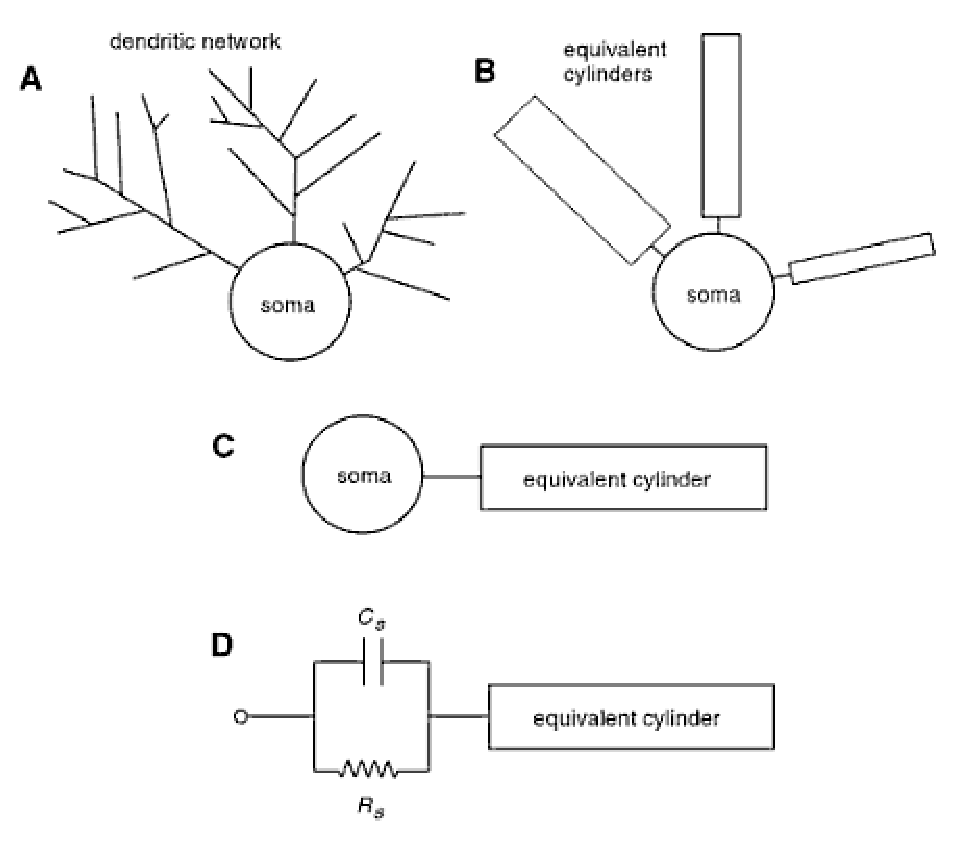
\includegraphics[height=6cm,
    angle=0]{./images/Rall_lumped_model.eps}}
\caption{Schematic diagram of the Rall lumped-soma model}
\label{fig:rall_lumpedmodel}
\end{figure}

In Rall's model, the membrane conductance is comprised of 3 components:
excitation, inhibition and resting.  Advances in experimental techniques had
proved both the electrotonic and active properties of neuron. The active
properties relate to the existence of a transient increase in transmembrane
potential at the soma, known as {\bf action potential}
(Sect.\ref{sec:AP-neuron}), revealed in details of these conductances.

\subsection{Cable model with compartments}
\label{sec:cylind-model-neur}

The extensively branched dendrite in the neuron is theoretically
modeled as a equivalent cylinder. Along the length of the dendritic
tree, there can be a variation in the densities of synaptic input.
\textcolor{blue}{Thus, to deal with spatio-temporal patterns of
  synaptic input, one possible choice was to split the dendrite tree
  into 5 or 10 regions of equal membrane surface area, including the
  soma},
as shown in Fig.~\ref{fig:cable_model}, (
\textcolor{blue}{the critical assumption is that everything in one
  region is uniformly distributed}),
then represent each region as a compartment (cylinder) in which
membrane capacity and several membrane conductances are treated as
lumped electric parameters~\citep{rall1967dts}.

\begin{figure}[hbt]
  \centerline{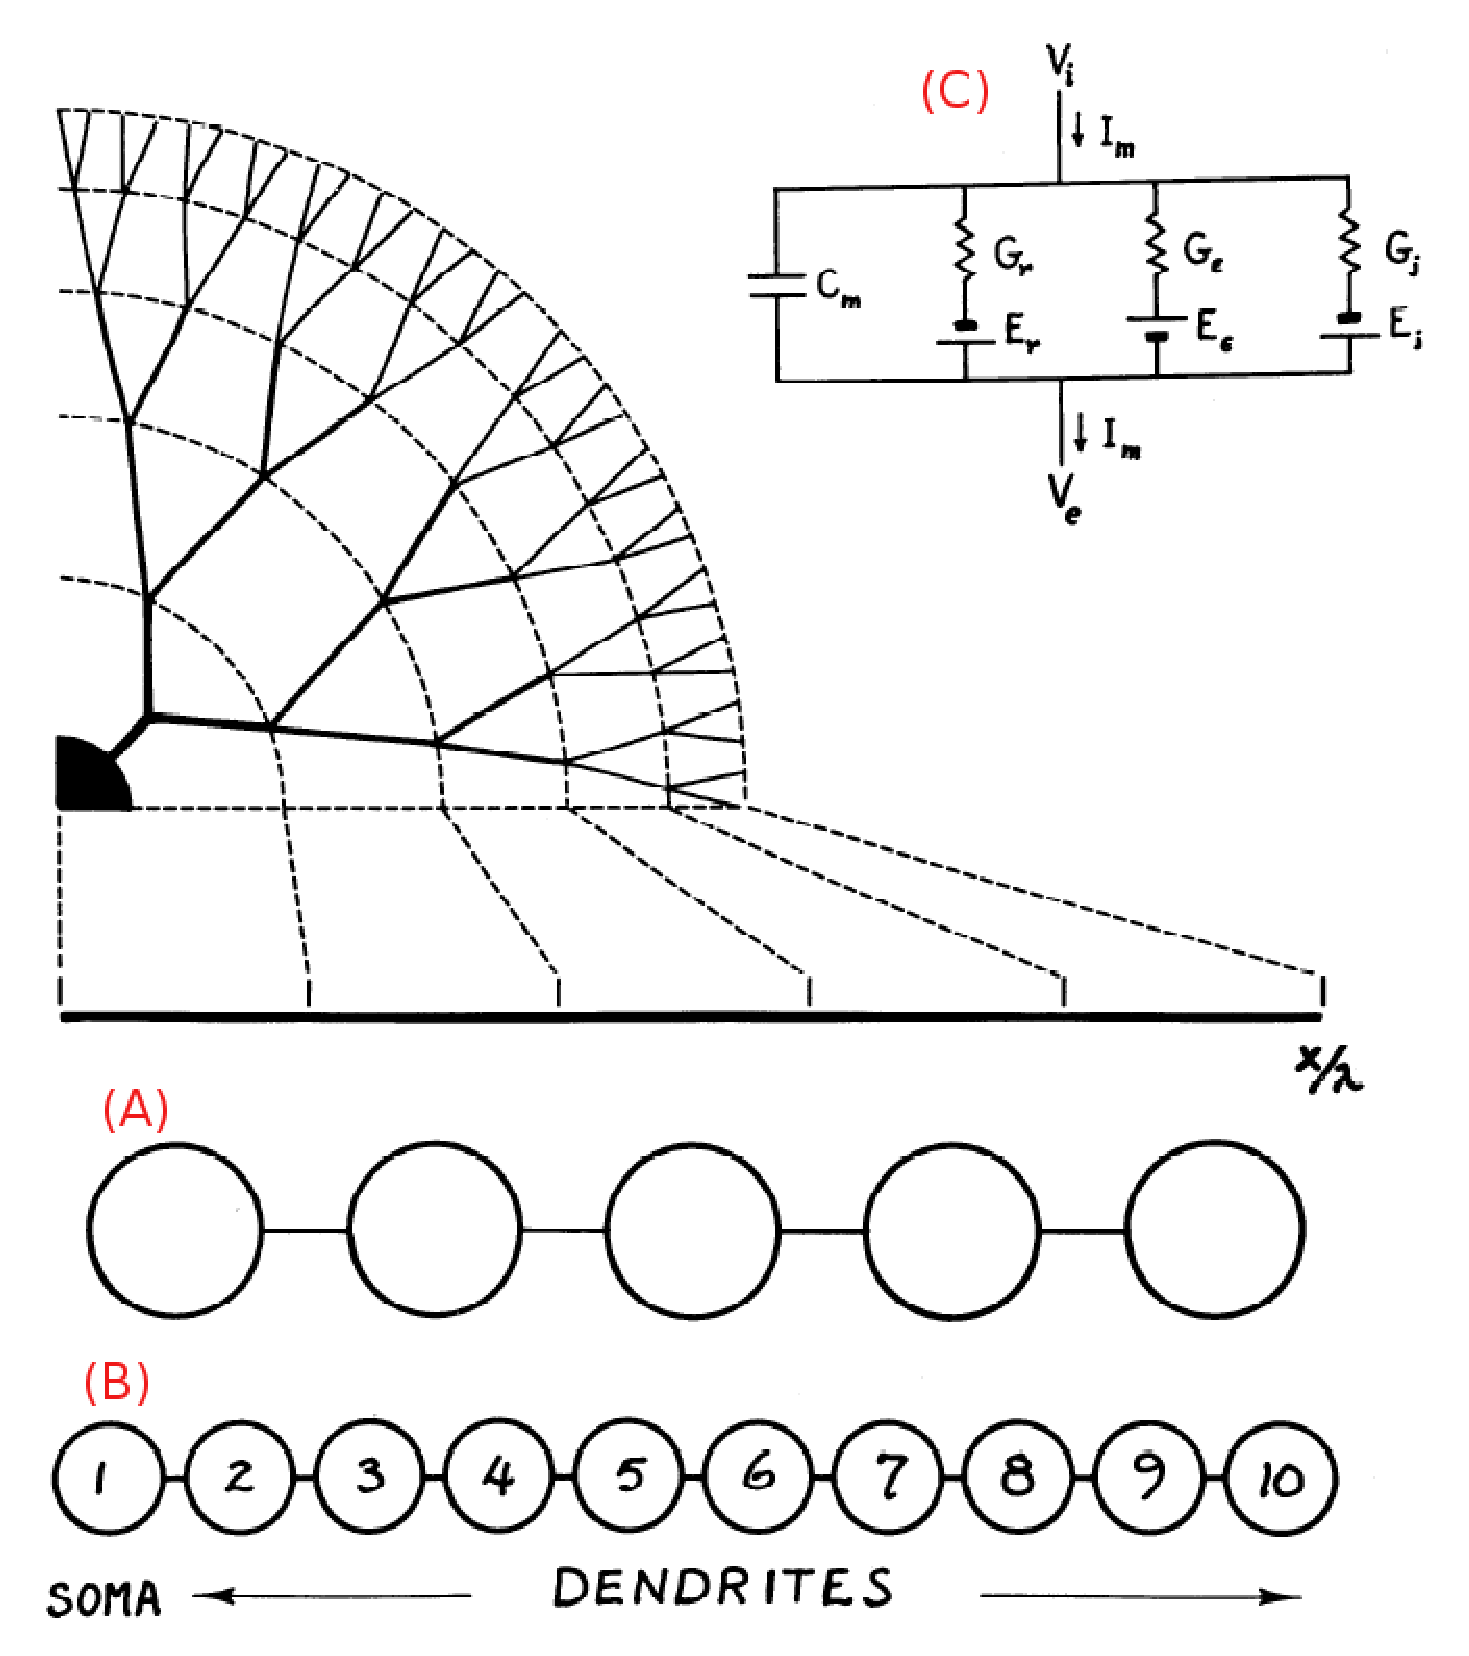
\includegraphics[height=8cm,
    angle=0]{./images/cable_model.eps}}
  \caption{Schematic diagram of a model representation for a pyramidal
    neuron: (A) 5-compartment model, (B) 10-compartment model; (C) The
    equivalent circuit for a single compartment}
\label{fig:cable_model}
\end{figure}

\textcolor{red}{The paper chose 10 compartments}, as shown in
Fig.~\ref{fig:cable_model}(B). Compartment 1 is the soma, the
compartment 10 is the lumping of most peripheral portions of all
dendrite trees belonging to this neuron model. Instead of using the
true length $l$, we use the concept of electrotonic distance, $Z$, so
that each compartment has the same $\Delta Z$.  In other words, the
true length is converted to $Z$ based on the characteristic length
$\lambda$ of the compartment
\begin{equation}
  \label{eq:402}
  Z = \int\limits_{0}^x \frac{dx}{\lambda}
\end{equation}
with $x$ is the physical distance along the cable, $\lambda$ is the
characteristic length (or {\bf length constant}) which changes with
branch diameter at the point of branching. 
$\Delta Z$ tells us the ``length'' of each compartment.

{\bf Example}: With $\Delta Z=0.2$, thus $Z=1.0$ is at compartment 6
and $Z=1.8$ at compartment 10.
\textcolor{red}{However, computations were commonly done with $\Delta
  Z =0.1$ or $\Delta Z = 0.4$.}

With 10 compartments, we have 10 different values for $\lambda_i$
($i=\overline{1..10}$).
\begin{eqnarray}
  \label{eq:405}
  \lambda = \sqrt{\frac{rR_m}{2R_i}}
\end{eqnarray}
with $r$ is the radius of the cylinder (change at each branching),
\begin{itemize}
\item $R_m$ is the specific membrane resistance
\item $R_i$ is the specific intracellular (axial) resistivity
\end{itemize} 
$R_m,R_i$ are experimentally determined and are assumed
to be the same for all compartments.  In the model, $\lambda$ is the
same for every point in a single compartment.  In an infinite length
cable model, $\lambda$ is called {\bf space constant}.

{\bf What is electrotonic potential?} - There are two types of
electrical potential: {\it electrotonic potential} (subthreshold
membrane potential) and {\it action potential} (transthreshold
membrane potential). Due to the passive transmission of electrical
impulse in dendrite, electrotonic potential is the topic.

% The latter is a propagated impulse, while the former is the
% non-propagated local potential caused by the local change in ionic
% conductance.

{\bf What is electrotonic length} - Electrotonic length is different
from electrotonic distance. Electrotonic length is defined as
$L=\frac{l}{\lambda}$ with $l$ is the length, from the soma to the end
of the compartment, while the definition of electrotonic distance can
be calculated at any point along the cylinder, not just the end point.


\subsection{Parameters in a compartment}
\label{sec:param-comp}

As studied in Chap.~\ref{sec:model-ion-channel}, a mathematical model is
a set of ordinary differential equations, which are normally linear
and of first-order; with some coefficients are constant, or some are
functions of time (e.g. those related to the synaptic conductance).

Rall didn't examined individual type of ionic channels particularly,
e.g. $\Na$, $\K$..., for simplicity he classified them into
excitatory and inhibitory conductance.  As you can see in
Fig.~\ref{fig:cable_model} (C), each compartment has 3 conductance
$G_r,G_\epsilon, G_j$, and one capacitor $C_m$. The three conductance
has three corresponding batteries $E_r, E_\epsilon, E_j$ and are all
constants. As $G_r$, the resting conductance, and $C_m$ are constant,
each compartment has 3 variables:
\begin{enumerate}
\item two independent variables:
  \begin{itemize}
  \item synaptic excitatory conductance $G_\epsilon$ $\rightarrow$ the
    synaptic excitatory intensity $\mathcal{E} =
    \frac{G_\epsilon}{G_r}$ ($G_r$ is the resting membrane
    conductance)
  \item synaptic inhibitory conductance $G_j$ $\rightarrow$ the
    synaptic inhibitory intensity $\mathcal{J} = \frac{G_j}{G_r}$
\end{itemize}

\item one dependent variables: the component's membrane potential
\end{enumerate}
In addition, there can be a fourth (independent) variable, the
external applied current $I_{app}$ to each compartment. 

Consider a single compartment, the membrane potential $V_m$ varies
within the range of resting potential $E_r$ to the excitatory
potential $E_\epsilon$. Thus, one way to measure the deviation of
$V_m$ from $E_r$ is to define a unitless quantity, called
{\bf membrane potential disturbance}
\begin{eqnarray}
  \label{eq:404}
  v = \frac{V_m-E_r}{E_\epsilon - E_r}
\end{eqnarray}
So, $v$ varies from 0 to 1. NOTE: $v=1$ when $\mathcal{E}$ very large
(excitatory signal), $\mathcal{J}$ small (no inhibitory signal), and
no applied current. However, peak values only reach at $v=0.01$ (small
EPSP), $v=0.1$ (large EPSP) in several simulation of synaptic
potentials which means that this is subthreshold potential.
%  $V_m=E_\epsilon$, i.e. in
% the absence of applied current, for $\mathcal{E}$ very large,
% $\mathcal{J}$ small). The negative value of $v$ represents membrane
% hyperpolarization. The limiting negative value is
% $\frac{E_j-E_r}{E_\epsilon-E_r}$ (i.e. in the absence of applied
% current and $\mathcal{J}$ much larger than $\mathcal{E}$).

% To facilitate the comparison between theoretical slope and
% experimental slope, a dimensionless quantity is define.
% \begin{eqnarray}
%   \label{eq:551}
%   (dv/dT)/v_p = \tau(dV/dt)/V_p
% \end{eqnarray}
% \textcolor{red}{Rall examined synaptic potential ($v\ll 1$), which is
%   not an action potential.  Thus, the synaptic intensity $\mathcal{E}$
%   was chosen to get the desired peak value for $v$ is 0.01 (small
%   excitatory postsynaptic potential - EPSP) or 0.1 (large EPSP) in the
%   soma compartment}.
% In the experiment data, a rising slope of 12V/sec for a synaptic
% potential of peak amplitude 4 mV. Then, for membrane time constant
% $\tau=5$ms, a dimensionless value $(dv/dt)/v_p$ is 15.

\subsection{Summary}
\label{sec:summary-2}

The model is designed to work with various neurons, thus dimensionless
variables are utilized extensively. Among them, only $V_m$ is the
dependent variable. Thus, the net depolarizing current density (loss
to the next regions and leak across the membrane) for a single
compartment is
\begin{eqnarray}
  \label{eq:549}
  C_m\frac{dV_m}{dt} = \left[C_m(E_\epsilon-E_r)/\tau\right] \frac{dv}{dT}
\end{eqnarray}
with $C_m=1\mu$F/cm$^2$, $(E_\epsilon-E_r)=70$mV, and $\tau=5$ms. The
factor enclosed by the square bracket is $14\mu$A/cm$^2$.
\textcolor{red}{With 10 compartment, we will have 10 first-order
  differential equation}.

We will combine with the linear cable equation
\begin{eqnarray}
  \label{eq:552}
  \frac{\partial V}{\partial T} + V  = \frac{\partial^2V}{\partial Z^2} + K\frac{\partial V}{\partial T}
\end{eqnarray}
with $V=V_m-E_r$.

\begin{itemize}
\item $\mathcal{E}$: one for each compartment
\item $\mathcal{J}$: one for each compartment
\item $v$ : the only dependent variable
\item $T=t/\tau$ the time course
\item $(dv/dT)/v_p$ (with $v_p$ is the peak of the synaptic potential,
  to compare the theoretical vs. experimental rising slope of synaptic
  potential)
\end{itemize}
% The state of a cylinder at any time is defined by 3 parameters. [ref
% 13]

% Its equivalent membrane circuit is given in [Fig]

% Similar to the membrane model given in Sec.~\ref{sec:models-membrane},
% $G_r$ is the resting membrane conductance in series with the resting
% membrane potential $E_r$, $G_\epsilon$ is the synaptic excitatory
% conductance; $G_r$ is the synaptic inhibitory conductance. 

{\bf NOTE}: The values of $E_r$ (membrane potential at rest),
$E_\epsilon$ (membrane potential at excitatory), and $E_j$ (membrane
potential at inhibitory).
\textcolor{red}{Assumptions: $E_\epsilon, E_r, E_j$ are assumed to be
  constant. In addition, the time course T is assumed to be independent
  of membrane potential and of applied current}.

% As $G_\epsilon$ and $G_j$ are independent variables, the synaptic
% excitatory intensity is $\mathcal{E}$ and synaptic inhibitory
% intensity $\mathcal{J}$ for each compartment is
% \begin{equation}
%   \label{eq:403}
%   \begin{split}
%       \mathcal{E} &= \frac{G_\epsilon}{G_r} \\
%       \mathcal{J} &= \frac{G_j}{G_r}
%   \end{split}
% \end{equation}
The two variables $\mathcal{E}, \mathcal{J}$ are known as
{\it synaptic input}. Due to the available of experimental data, the
synaptic conductance change smoothly via the transient synaptic
function which can be either ``fast'', ``medium'', and
``slow''\footnote{how long to reach its peak $v=1$}
\begin{eqnarray}
  \label{eq:550}
  F(T) = \frac{T}{T_p} \exp(1-\frac{T}{T_p})
\end{eqnarray}
with $T_p=0.02$ (fast), $T_p=0.04$ (medium), and $T_p=0.092$
(slow). F(T) start from 0 (at T=0), increase to 1 (at $T=T_p$), and
then decrease to zero again ($T\rightarrow \infty$). The area under
the entire curve equal $eT_p$ (where $e$ is the base of the natural
algorithm). 

The half-width is defined as the duration between the two points whose
values are half of the peak. This value provides a quantity to
estimate the shape of the EPSP. 
% Excitation deviating from the resting potential is measured via the
% dimensionless variable $v$
% \begin{eqnarray}
%   \label{eq:404}
%   v = \frac{V_m-E_r}{E_\epsilon - E_r}
% \end{eqnarray}
% with $v$ from negative to 1 (when $V_m=E_\epsilon$, i.e. in the
% absence of applied current, for $\mathcal{E}$ very large,
% $\mathcal{J}$ small). The limiting negative value is
% $\frac{E_j-E_r}{E_\epsilon-E_r}$ (i.e. in the absence of applied
% current and $\mathcal{J}$ much larger than $\mathcal{E}$).

% Peak amplitudes of $v=0.01$ and $v=0.1$ 

\subsubsection{Synaptic input at different compartments}
\label{sec:synaptic-input-at}


\subsubsection{Effect of fast/medium/slow synaptic input transient}
\label{sec:effect-fastm-synapt}


\subsubsection{Effects of electrotonic length}
\label{sec:effects-electr-lengt}

Electrotonic length of $\Delta Z = 0.2$ or $\Delta Z = 0.1$ was being
used to test. A good approximation: ``doubling $\Delta Z$
approximately doubles the time-to-peak value obtained for a given
input compartment''. 

SUMMARY: One cannot induce the location (at which compartment) and
time course of synaptic input just by looking at EPSP curve alone. If
we use multiple input locations, the combination can greatly increase
the variety in the shape of EPSP (at the soma, i.e. first
compartment).


\begin{eqnarray}
  \label{eq:532}
  \frac{dv/dT}{v_p} = \frac{\tau dV/dt}{V_p}
\end{eqnarray}
with $V=V_m-E_r$ and $V_p$ is the peak value.

% Synaptic input transient function
% \begin{eqnarray}
%   \label{eq:533}
%   F(T) = (T/T_p) \exp^{1-T/T_p}
% \end{eqnarray}
% \begin{enumerate}
% \item For fast input transient: it reaches the peak at $T=0.02$, and
%   half-width (duration reach half of the peak) at $T=0.049$
% \item For medium input transient: it reaches the peak at $T=0.04$, and
%   half-width (duration reach half of the peak) at $T=0.098$
% \item For slow input transient: it reaches the peak at $T=0.092$, and
%   half-width (duration reach half of the peak) at $T=0.225$

% \end{enumerate}


References:
\begin{enumerate}
\item A good reference to the cable theory and model is Chapter 4 of
  Johnston and Wu~\citep{johnston1994fcn}.
\end{enumerate}

\section{Dodge-Cooley model (1973)}
\label{sec:dodge-cooley-model}

A motoneuron has typically 7 large dendrite leaving the soma. They
branch profusely to increase the surface area on which other neurons
can make synaptic connection. When an action potential (AP), starting
from the soma, reach the terminal of the synapse, it triggers the
release of packages of neurotransmitter, in unit (called
quantum). Each quantum when reaching the postsynaptic, contribute a
postsynaptic potential $p$ to the other cell.  As the axon can be
long, during the transmission pathway along the axon, there are
amplifier known as {\bf nodes of Ranvier}. Thus, this is called an
active process.


A single cell may receive many of the postsynaptic potential from many
of its synaptic connections and will passively propagate to the neuron
soma\footnote{the name ``passive'' as there is no amplifier}. If the
total postsynaptic potential is large enough, an action potential can
be triggered at the soma and the signal is transmitted to other cells
\citep{dodge1973apm}.

\section{Traub-Llinas model (1977)}
\label{sec:Traub-Llinas-1977}

~\citep{traub1977sdi}. 

%%% Local Variables: 
%%% mode: latex
%%% TeX-master: "mainfile"
%%% End: 
